\chapter{Aufgabe 3: Skalarprodukt}

Die Abbildungen~\ref{fig:aufgabe3} zeigen die Laufzeiten der sequentiellen Ausführung und der parallelen Ausführungen mit 1, 2, 4, 8 und 16 Threads und Tabelle~\ref{tab:aufgabe3_tab} listet diese auf. Die sequentielle Ausführung und die ,,parallele Ausführung'' mit einem Thread brauchten im Wesentlichen gleich viel Zeit, was zu erwarten war, da eine parallele Ausführung mit einem Thread das gleiche ist wie eine sequentielle Ausführung. Weiterhin kann man beobachten, dass die Laufzeit mit der Zunahme von Threads bis zur Zahl 8 sinkt und für 16 Threads wieder etwas ansteigt. Aus der doppellogarithmischen Darstellung in Abb.~\ref{fig:aufgabe3_logplot} kann man erahnen, dass die Abnahme der Laufzeit logarithmisch erfolgt.

\begin{figure}[htbp]
 \centering 
 \begin{subfigure}{.49\textwidth}
  \centering 
  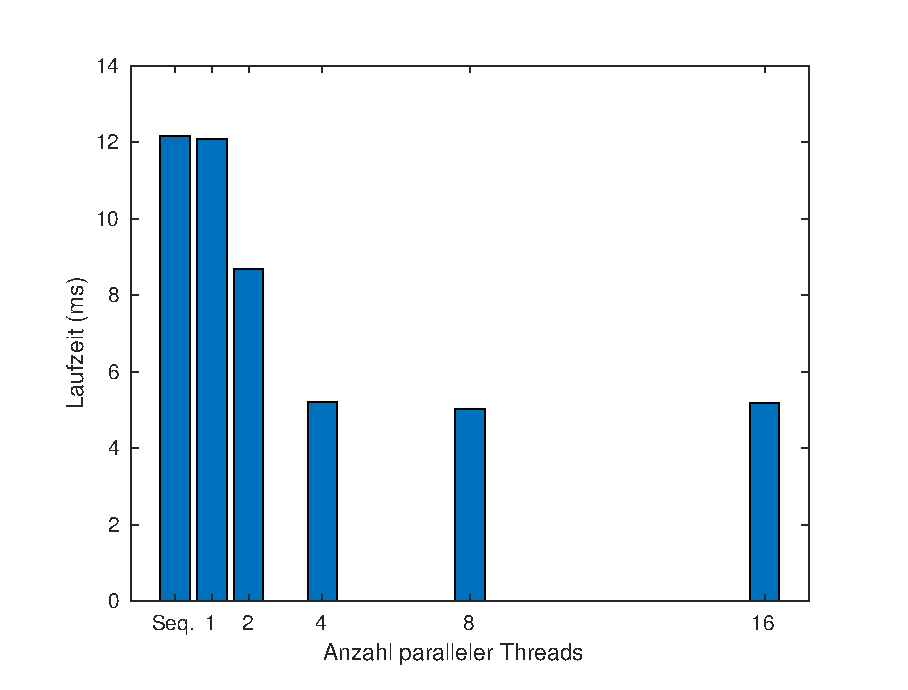
\includegraphics[width=1\textwidth]{img/aufgabe3_barplot.eps}
  \caption{Säulendiagramm.}
  \label{fig:aufgabe3_barplot}
 \end{subfigure}
%
 \begin{subfigure}{.49\textwidth}
  \centering 
  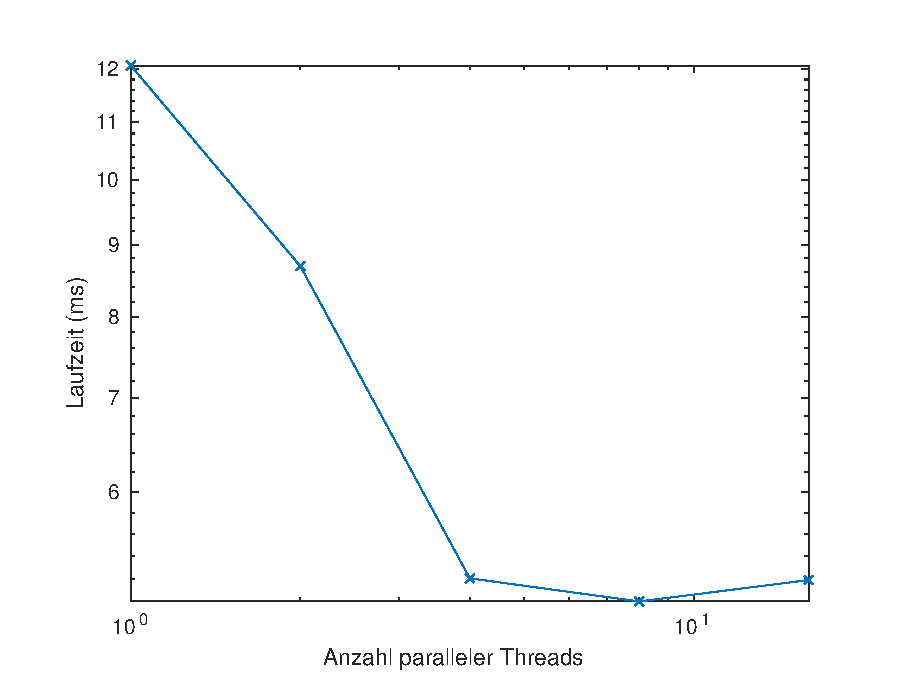
\includegraphics[width=1\textwidth]{img/aufgabe3_logplot.eps}
  \caption{Doppellogarithmische Darstellung.}
  \label{fig:aufgabe3_logplot}
 \end{subfigure}
\caption{Laufzeiten für sequentielle Ausführung und parallele Ausführung mit 1, 2, 4, 8, 16 Threads von dotproduct.}
\label{fig:aufgabe3}
\end{figure}

\begin{table}[h]
\caption{Laufzeiten für dotproduct.}
\centering 
 \begin{tabular}{|l|r|}
  \textbf{Ausführungsart} & \textbf{Benötigte Zeit (ms)} \\ \hline
  Sequentiell & 12.1569 \\
  Parallel mit 1 Thread & 12.0733 \\
  Parallel mit 2 Threads & 8.6913 \\
  Parallel mit 4 Threads & 5.2090 \\
  Parallel mit 8 Threads & 5.0150 \\
  Parallel mit 16 Threads & 5.1945
 \end{tabular}
 \label{tab:aufgabe3_tab}
\end{table}
